\documentclass[progressbar=head]{beamer}
\usetheme{dresden}
\usepackage[utf8]{inputenc}
\usepackage[english]{babel}
\usepackage{amsmath}
\usepackage{amsfonts}
\usepackage{amssymb}
\usepackage{graphicx}

\usepackage{ mathrsfs }

\usepackage{ bbold }

%\usepackage{cite}

\usepackage{caption}

% packages
\usepackage{mdframed}

%for links
%\usepackage{hyperref}

% for units
\usepackage{siunitx}

% for the vector on ones
\usepackage{bbm}

% to get the units correctly for printing
%\usepackage{layouts}

% for commenting multiple lines efficiently
\usepackage{comment}

% for fancy tables
\usepackage{booktabs}

%\usepackage{esint}

%\usepackage{mathtools}

% for bibliography
\usepackage[style=authoryear]{biblatex}
\addbibresource{refs.bib}

\usepackage{csquotes}

%%%%%%%%%%%%%%%%%%%%%%%%%%%%%%%%%%%%%%%%%%%%%%%%%%%%%%%%%%%%%%%%%%%%%%%%%%%%%%%%%%%%%%
%%%%%%%%%%%%%%%%%%%%%%%%%%%%%%%%%%%%%%%%%%%%%%%%%%%%%%%%%%%%%%%%%%%%%%%%%%%%%%%%%%%%%%

\title{New Methods in Electrical Source Imaging Based on EEG and Post-Mortem Pathology Data}
\date{August 7, 2024}
\author{Julio Cesar Enciso-Alva}
\institute{University   of Texas at Arlington}

%%%%%%%%%%%%%%%%%%%%%%%%%%%%%%%%%%%%%%%%%%%%%%%%%%%%%%%%%%%%%%%%%%%%%%%%%%%%%%%%%%%%%%
%%%%%%%%%%%%%%%%%%%%%%%%%%%%%%%%%%%%%%%%%%%%%%%%%%%%%%%%%%%%%%%%%%%%%%%%%%%%%%%%%%%%%%

\allowdisplaybreaks

%\definecolor{mygreen}{rgb}{0,0.6,0}
%\definecolor{mygray}{rgb}{0.5,0.5,0.5}
%\definecolor{mymauve}{rgb}{0.58,0,0.82}


%\addtocontents{toc}{\noindent\mbox{Chapter}\hfill\mbox{Page}}%

%\renewcommand{\listalgorithmname}{LIST OF ALGORITHMS}
%\addtocontents{loa}{\noindent\mbox{Algorithm}\hfill\mbox{Page}}
%\numberwithin{algorithm}{chapter}

\newcommand{\ts}{\textsuperscript}
\newcommand{\Supp }{\rm Supp}
\newcommand{\pa }{\partial }
\newcommand{\f}{\frac}
\newcommand{\me}{\mathrm{e}}
\newcommand{\mi}{\mathrm{i}}
\newcommand{\mpi}{\mathrm{\pi}}
\newcommand{\msh}{\mathrm{sinh}\,}
\newcommand{\mch}{\mathrm{cosh}\,}
\newcommand{\mth}{\mathrm{tanh}\,}

%%%%%%%%%%%%%%%%%%%%%%%%%%%%%%%%%%%%%%%%%%%%%%%%%%%%%%%%%%%%%%%%%%%%%%%%%%%%%%%%%%%%%%
%%%%%%%%%%%%%%%%%%%%%%%%%%%%%%%%%%%%%%%%%%%%%%%%%%%%%%%%%%%%%%%%%%%%%%%%%%%%%%%%%%%%%%

%% PARENTHESIS

\newcommand{\sset}[1]{ \left\{ #1 \right\} }
\newcommand{\ppar}[1]{ \left( #1 \right) }
\newcommand{\spar}[1]{ \left[ #1 \right] }

\newcommand{\abss}[1]{ \left| {#1} \right| }

\newcommand{\nnorm}[1]{\left\lVert #1 \right\rVert}

%% MATRICES

%\newcommand{\R}{\mathbb{R}}
%\newcommand{\ones}[1]{ \mathbbm{1}_{N_{#1}} \mathbbm{1}_{N_{#1}}^\intercal }

\newcommand{\ones}{\mathbbm{1}}

\newcommand{\trans}{^T}
\newcommand{\iinv}{^{-1}}
\newcommand{\pinv}{^\dagger}

\newcommand{\diag}[1]{\text{diag}\ppar{ #1 }}

%% PROBABILITY

\newcommand{\prob}{\text{Prob}}
\newcommand{\given}{\;\middle|\;}

\newcommand{\vvar}[1]{\text{Var}\ppar{#1}}
\newcommand{\ccov}[1]{\text{Cov}\ppar{#1}}

%\newcommand{\ccon}[2]{\left\phantom{(} #1 \mathrel{}\middle|\mathrel{} #2 \right\phantom{)}}

%% OPTIMIZATION

\DeclareMathOperator*{\argmax}{arg\,max}
\DeclareMathOperator*{\argmin}{arg\,min}

%% BIG LETTERS

\newcommand{\J}{\mathbf{J}}
\newcommand{\Y}{\mathbf{Y}}
\newcommand{\G}{\mathbf{G}}

\newcommand{\PA}{\mathbf{P}}
\newcommand{\SA}{\mathbf{S}}
\newcommand{\AAA}{\mathbf{A}}

\newcommand{\RA}{\mathbf{R}}
\newcommand{\BA}{\mathbf{B}}

\newcommand{\U}{\mathbf{U}}
\newcommand{\N}{\mathbf{N}}

\newcommand{\rr}{\mathbf{r}}
\newcommand{\sa}{\mathbf{s}}
\newcommand{\dd}{\mathbf{d}}

\newcommand{\ee}{\mathbf{e}}
\newcommand{\mm}{\mathbf{m}}

\newcommand{\V}{\mathbf{V}}

\newcommand{\Gbar}{\overline{\mathbf{G}}}
\newcommand{\Ybar}{\overline{\mathbf{Y}}}

%% BASICS

\newcommand{\R}{\mathbb{R}}

\newcommand{\id}{\mathbf{I}}
\newcommand{\norm}{\mathcal{N}}

%% DEPRECATED

\newcommand{\GAM}{\mathbf{\Gamma}}
\newcommand{\SIG}{\mathbf{\Sigma}}
\newcommand{\ga}{\pmb{\gamma}}

\newcommand{\jt}{\mathbf{j}}

\newcommand{\W}{\mathbf{W}}

\newcommand{\LL}{\mathbf{\Lambda}}


%%%%%%%%%%%%%%%%%%%%%%%%%%%%%%%%%%%%%%%%%%%%%%%%%%%%%%%%%%%%%%%%%%%%%%%%%%%%%%%%%%%%%%
%%%%%%%%%%%%%%%%%%%%%%%%%%%%%%%%%%%%%%%%%%%%%%%%%%%%%%%%%%%%%%%%%%%%%%%%%%%%%%%%%%%%%%

%\def\SPSB#1#2{\rlap{\textsuperscript{#1}}\SB{#2}}
%\def\SP#1{\textsuperscript{#1}}
%\def\SB#1{\textsubscript{#1}}


%%%%%%%%%%%%%%%%%%%%%%%%%%%%%%%%%%%%%%%%%%%%%%%%%%%%%%%%%%%%%%%%%%%%%%%%%%%%%%%%%%%%%%
%%%%%%%%%%%%%%%%%%%%%%%%%%%%%%%%%%%%%%%%%%%%%%%%%%%%%%%%%%%%%%%%%%%%%%%%%%%%%%%%%%%%%%

\begin{document}

\AtBeginSection[]{
  \begin{frame}
  \vfill
  \centering
  \begin{beamercolorbox}[sep=8pt,center,shadow=true,rounded=true]{title}
    \usebeamerfont{title}\insertsectionhead\par%
  \end{beamercolorbox}
  \vfill
  \end{frame}
}



{
%\metroset{background=dark}
\maketitle

\begin{frame}%{Overview}
\tableofcontents[pausesections,hideothersubsections]
\end{frame}
}

%\addcontentsline{toc}{section}{Foreword}

\begin{frame}{Biographic Statement}
\begin{itemize}
\item I was born and raised on Pachuca, a small city on central Mexico.
\item Studied Applied Math at UAEH (Hidalgo State University).
\end{itemize}
\begin{figure}
\centering
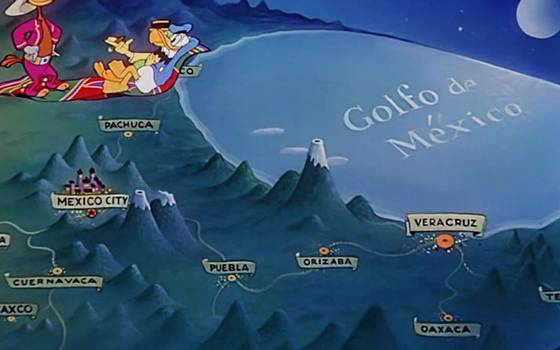
\includegraphics[width=0.7\linewidth]{./img_dev3/caballeros}
\end{figure}
\end{frame}

\begin{frame}{Biographic Statement}
Hi to my family.
\begin{figure}
\centering
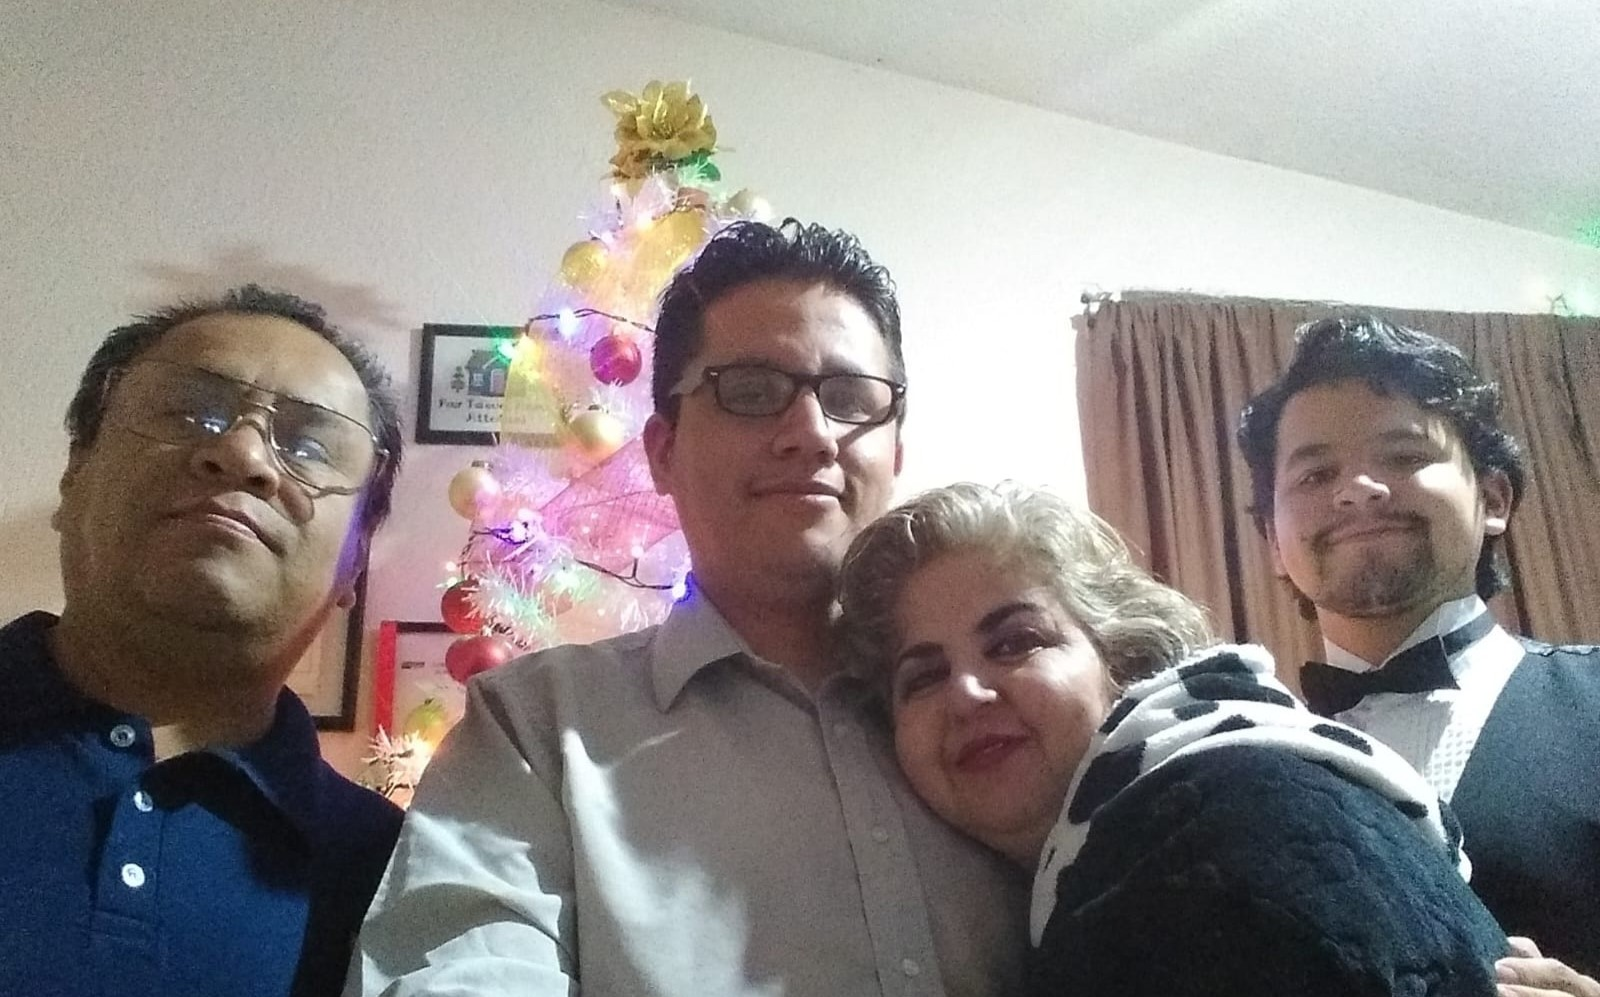
\includegraphics[width=0.75\linewidth]{./img_dev3/family}
\end{figure}
\end{frame}


{
%\metroset{background=dark}
\section{Introduction}
}

\begin{frame}{Introduction}
\begin{itemize}
\item Multiple EEG patterns have been found to be related to normal and pathological states \footfullcite{niedermeyer2011niedermeyer}. 
\item Electrical Source Imaging (ESI) is a framework to locate the neural sources of electric/magnetic activity.
\item EEG has high resolution in time, low resolution in space. 
\item ESI is ill-posed, in the sense of Hadamard.
\end{itemize}
%\begin{figure}
%\centering
%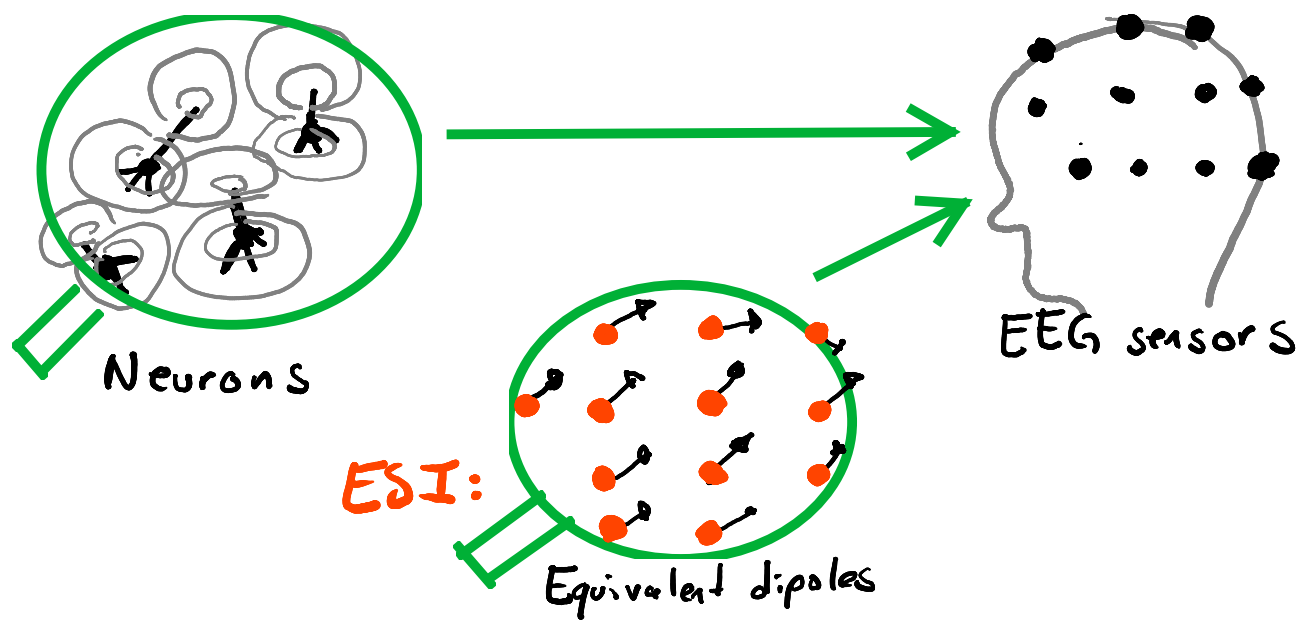
\includegraphics[width=0.6\linewidth]{./img_oldbeamer/sketch03}
%\end{figure}
\end{frame}




\begin{frame}{Previous Results}
Electrical Source Imaging was used; for example, 
to study epilepsy caused by Glucose transporter type I deficiency (G1D) \footfullcite{dr_pascal}.
\end{frame}

{
%\metroset{background=dark}
\section{Forward Problem}
}

\begin{frame}{Neuron Dipoles}
\begin{itemize}
\item A single post-synaptic potential 
acts like an electric dipole and
produces an electric scalar field, $V$. 
%This can be modeled as a single dipole.
\item Each single neuron is too small to produce a significant change. The combined action of all neurons produces a large current density field.
\item EEG electrodes are located finite set at $\sa_1, \sa_2, \dots, \sa_M$.
\item EEG measures a difference in scalar electric field, $V$,
\begin{equation}
\Y(m) = V\ppar{\sa_m} - V\ppar{\sa_\text{ref}}
\end{equation}
with $\sa_\text{ref}$ an `electrical neutral' point.
\end{itemize}
\end{frame}

\begin{frame}{Equivalent Dipoles}
\begin{itemize}
\item \alert{Key assumption:} Consider a finite set of \textbf{distributed dipoles}, which produce the same electric field observe by the EEG.
\item Location of these dipoles is known: $\dd_1, \dots, \dd_N$.
%\item `Silent activity' occurs when singular neuron dipoles don't fire coherently. It can't be observed using EEG.
\item Consider the $n$-th dipole as $\rho_n \ee_n$ with $\nnorm{\ee_n}_2=1$.
\end{itemize}
\begin{figure}
\centering
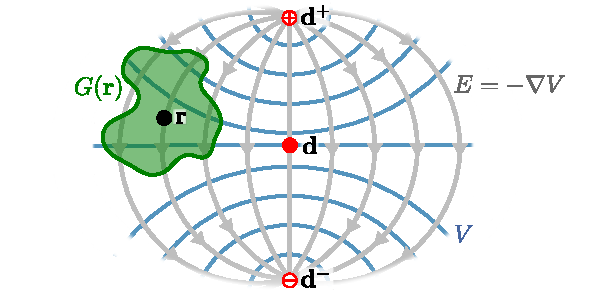
\includegraphics[width=0.45\linewidth]{./img/CurrDensField}
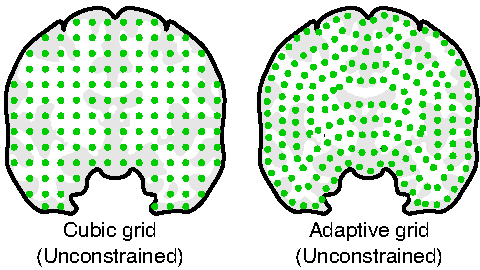
\includegraphics[width=0.45\linewidth]{./img/Pregions_pic_radial_v2}
\end{figure}
\end{frame}

\begin{frame}{Green Equation for 1 dipole + 1 sensor}
\begin{itemize}
\item Consider the $m$-th EEG sensor and the $n$-th equivalent dipole.
\item The electrical potential field, $V$, follows
\begin{equation}
\nabla \cdot\ppar{\sigma(\rr)\, \nabla V(\rr) } = 
\rho\spar{ \delta\ppar{\rr-\ee_n^+} + \delta\ppar{\rr-\ee_n^-} }
\label{eq:01}
\end{equation}
with $\sigma\ppar{\rr}$ the conductivity.
\item For the isotropic case, $\sigma\ppar{\rr}= \kappa \id$, equation \ref{eq:01} reduces to 
\begin{equation}
\kappa\, \Delta { V(\rr) } = 
\rho\spar{ \delta\ppar{\rr-\ee_n^+} + \delta\ppar{\rr-\ee_n^-} }
\label{eq:02}
\end{equation}
\end{itemize}
\end{frame}

\begin{frame}{Green Equation: Domain}
\begin{itemize}
\item We use the 4-sphere model: the domain is 4 media (brain, CSF, skull, head) with regional-constant conductivity.
\item Solutions must be regular:
%\begin{equation}
$\sigma(\bullet)\, V(\bullet) \in C^1 \ppar{\mathcal{M}_1 \cup \dots, \cup \mathcal{M}_4}$.
%\end{equation}
\item Air is non-conductive, so we use reflective boundary conditions
\begin{equation}
\kappa\, \nabla V(\rr) \cdot \mathbf{n} = 0, \text{ for } \rr\in \mathcal{M}_1.
\end{equation}
\begin{figure}
\centering
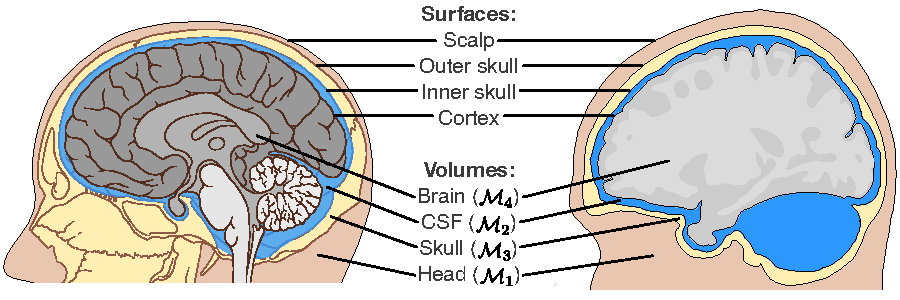
\includegraphics[width=0.8\linewidth]{./img/HeadSurfacesVolumes}
\end{figure}
\end{itemize}
\end{frame}

\begin{frame}{Green Equation for $M$ sensors + $N$ dipole}
\begin{itemize}
\item Consider $\tilde{V}_n$ the solution to 
\begin{equation}
\kappa\, \Delta { \tilde{V}_n(\rr) } = 
{ \delta\ppar{\rr-\ee_n^+} + \delta\ppar{\rr-\ee_n^-} },
\end{equation}
\item The electrical scalar field from all the equivalent dipoles, at the $m$-th sensor, is given by
\begin{equation}
V(\sa_m) = \sum_{n=1}^N \rho_n \tilde{V}_n \ppar{\sa_m}
=
\begin{bmatrix}
\tilde{V}_1 \ppar{\sa_m} &
\cdots &
\tilde{V}_N \ppar{\sa_m}
\end{bmatrix}
\begin{bmatrix}
\rho_1 \\ \vdots \\ \rho_N
\end{bmatrix}
\label{eq:stack}
\end{equation}
\end{itemize}
\end{frame}

\begin{frame}{Resulting Model}
\begin{itemize}
\item Observation from $M$ sensors can be stacked as
\begin{equation}
\begin{bmatrix}
V\ppar{\sa_1}
\\
V\ppar{\sa_2}
\\
\vdots \\
V\ppar{\sa_M}
\end{bmatrix}
=
\begin{bmatrix}
\tilde{V}_1 \ppar{\sa_1} &
\tilde{V}_2 \ppar{\sa_1} &
\cdots &
\tilde{V}_N \ppar{\sa_1} \\
\tilde{V}_1 \ppar{\sa_2} &
\tilde{V}_2 \ppar{\sa_2} &
&
\tilde{V}_N \ppar{\sa_M} \\
\vdots &  & \ddots & \vdots \\
\tilde{V}_1 \ppar{\sa_M} &
\tilde{V}_2 \ppar{\sa_M} &
\cdots &
\tilde{V}_N \ppar{\sa_M}
\end{bmatrix}
\begin{bmatrix}
\rho_1 \\ \rho_2 \\ \vdots \\ \rho_N
\end{bmatrix}
\end{equation}
\item Such equation can be summarized as
\begin{equation}
\Y = \G \SA
\end{equation}
with $\G$ referred to as the \alert{leadfield matrix}.
\item $\Y$ depends entirely on EEG data, $\G$ can be computed from anatomical data, and $\SA$ is to be found.
\end{itemize}
\end{frame}

\begin{frame}{Case of Unknown Orientation}
\begin{itemize}
%\item We may assume that dipoles at the cortex surface are orthogonal to it. This assumption is motivated by physiological observations. 
\item If the dipoles' orientation is unknown, each dipole can be projected into canonical coordinates, so
\begin{equation}
\rho_n\, \ee_n =
\rho_n^x\, \ee_n^x + \rho_n^y\, \ee_n^y + \rho_n^z\, \ee_n^z.
\end{equation}
\item To recover the original interpretation, find $\abss{\rho_n}$.
\begin{figure}
\centering
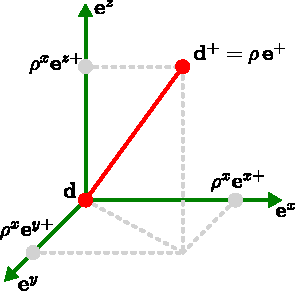
\includegraphics[width=0.4\linewidth]{./img/OrthDecomp}
\end{figure}
\end{itemize}
\end{frame}

\begin{frame}{Practical considerations}
Steps to solve the Forward Problem:
\begin{enumerate}
\item Start with anatomic MRI from subject (or template) and locations of EEG electrodes.
\item Segmentation: Identify relevant volumes.
\item Reconstruction triangulated surfaces.
\item Generate locations of distributed dipoles.
\item Solve equation \ref{eq:02} to compute $\G$.
\end{enumerate}

\end{frame}

\begin{frame}{Typical Pipeline for ESI}
\begin{figure}
\centering
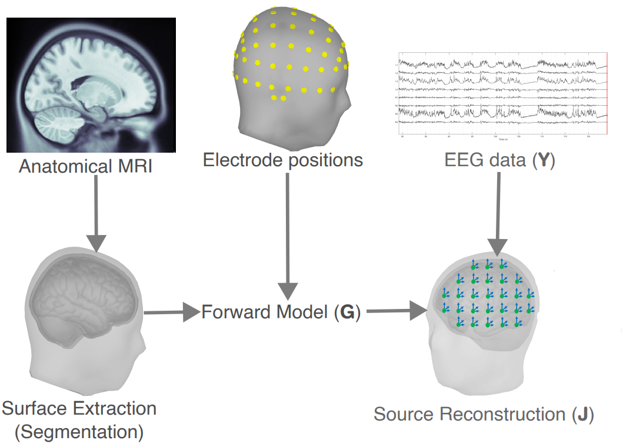
\includegraphics[width=0.7\linewidth]{./img_dev/pipeline}
\end{figure}
\end{frame}


{
%\metroset{background=dark}
\section{Inverse Problem}
}

\begin{frame}{Literature Review}
Electrical Source Imaging (ESI) consist in estimating $\SA$ from the equation
\begin{equation}
\Y = \G\, \SA + \varepsilon
\end{equation}
with $\Y\in \R^{M\times T}$ is given, $\G\in \R^{kN\times T}$ is given with $k\in \sset{1,3}$, and $\varepsilon$ is a noise term.\\

Many methods have been described to accomplish this task.
%
Asadzadeh et al. reported 41 different ESI algorithms between 1970 and June 2019, most of which were used to study clinical conditions.
\end{frame}

\begin{frame}{Weighted Minimal Norm Estimator (wMNE)}
Dipoles near the sensors are often over-represented in the inverse solution. The weight $W$ is used to alleviate that.
\begin{align}
\hat{\SA}_\text{wMNE} 
&=
\G\trans
\ppar{\G \ppar{W\trans W}\iinv \G\trans + \lambda\, \id_M}\iinv \Y
\\
W &=
\diag{ \nnorm{\G(:,1)}_2, \nnorm{\G(:,2)}_2, \dots, \nnorm{\G(:,N)}_2 }
\end{align}
\end{frame}


\begin{frame}{sLORETA\footfullcite{sloreta}}
%sLORETA  considers a small variant of the minimization function
\begin{equation}
    \hat{\mathbf{S}} = \argmin_{\mathbf{S}}\, \nnorm{\G \mathbf{S}-\Y-c \mathbb{1}}_2^2 + \lambda\, \nnorm{\mathbf{S}}_2^2
\end{equation}
with $\mathbb{1}=\{1\}^{M\times 1}$.
If $\Y$ is re-referenced to average, then $c=0$.


The solution is given by
\begin{equation}
    \hat{\mathbf{S}}_{\text{sLORETA}}
    =
    \G^T H\spar{H\, \G\, \G^T H+ \lambda H}^{\dagger}
    \mathbf{M}^\delta
\end{equation}
with $H$ an averaging operator constructed as
\begin{equation*}
    H = \id - \ppar{\mathbb{1} \mathbb{1}^T}/\ppar{\mathbb{1}^T \mathbb{1}}
\end{equation*}

\end{frame}

\begin{frame}{Multivariate Source Prelocalisation (MSP)\footfullcite{mattout2005multivariate}}
Dipoles near the sensors are often over-represented in the inverse solution. The weight $W$ is used to alleviate that.
\begin{align}
\hat{\SA}_\text{MSP} 
&=
\G\trans
\ppar{\G \ppar{W\trans W}\iinv \G\trans + \lambda\, \id_M}\pinv \Y
\end{align}

The weight $W$ is obtained by (1) projecting $\G$ into a small number of singular values, obtaining $\bar{\G}$, and then (2) obtaining the correlations of $\bar{\G} \Y$.
\end{frame}


\subsection{Performance Metrics}

\begin{frame}{Performance Metrics: Localization Error}
The location of an estimated source patch is defined using the center of mass,
\begin{equation}
    \hat{\mm}_p = 
\frac{\displaystyle \sum_{n\in \mathcal{I}_p} \nnorm{\hat{\SA}(n)}_2^2 \rr_n }{\displaystyle \sum_{n\in \mathcal{I}_p} \nnorm{\hat{\SA}(n)}_2^2}
\end{equation}

Distance Localisation Error (DLE) is defined as
\begin{equation}
\text{DLE} = 
\frac{1}{P} \sum_{p=1}^P \nnorm{ \mm_p - \hat{\mm}_p }_2
\label{def:DLE}
\end{equation}
\end{frame}

\begin{frame}{Performance Metrics: Spatial Dispersion}
Proposed by Molins et al \footfullcite{molins2008quantification}, 
\begin{equation}
\text{SD}
=
\ppar{
\frac{ \displaystyle
\sum_{p=1}^P \sum_{n\in \mathcal{I}_p} \nnorm{\hat{\SA}(n)}_2^2\, \nnorm{\rr_n-\mm_p} }{\sum_{n=1}^N \nnorm{\hat{\SA}(n))}_2^2}
}^{1/2}
\end{equation}

In some sense, Spatial Dispersion (SD) behaves a variance in space.
\end{frame}

\begin{frame}{Performance Metrics: AUROC and Avg. Precision}
Area Under Receiver-Operator Curve (AUROC) measures how good is a classifier.

In the context of ESI, the estimated labels are defined as
\begin{align}
\mathcal{E}_\beta(n)
&=
\begin{cases}
1, &\text{if }
\nnorm{\hat{\SA}(n)}_2 \geq \beta \max_{n'}\sset{\nnorm{\hat{\SA}(n')}_2}
\\
0, &\text{otherwise}
\end{cases}
\end{align}

\begin{itemize}
\item AUROC is defined using the parametric curve True-Positive-Rate vs False-Positive Rate.
\item Average Precision is defined using the parametric curve Recall vs Precision
\end{itemize}

\end{frame}

\begin{frame}{Performance Metrics: AUROC}
\begin{figure}
\centering
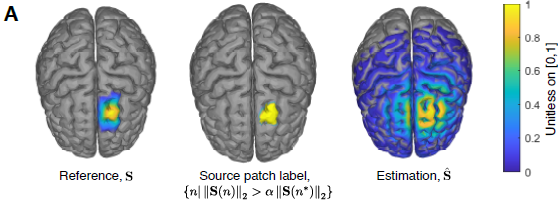
\includegraphics[width=0.8\linewidth]{./img_dev3/auroc1}
\end{figure}
\end{frame}

\begin{frame}{Performance Metrics: AUROC}
\begin{figure}
\centering
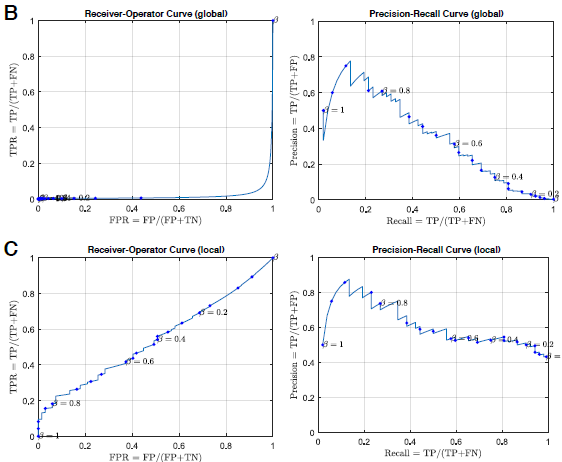
\includegraphics[width=0.6\linewidth]{./img_dev3/auroc2}
\end{figure}
\end{frame}

{
%\metroset{background=dark}
\section{Proposed Method}
}

\begin{frame}{Assymetric Multi-modal Data Analysis}
When dealing with multiple `modalities' of data, A and B, the information from B is incorporated during the analysis of A.

We consider the case where a region, identified using an histochemical test, is known to produce a higher background activity.
%
We refer this region to as the P-region.

Now the goal is to incorporate the P-region into the ESI model with the aim of improving the results. 
\end{frame}

\begin{frame}{Model Assumptions}
\begin{itemize}
\item The model equation, $\Y = \G \ppar{\SA + \varepsilon}$, is unchanged. 
\item We use $\SA \in \R^{N\times 1}$ or $\SA \in \R^{3N\times 1}$ as needed. 
\item Only one time-point is considered.
\item P-regions are encoded into the following matrix
\begin{equation}
\PA(n,k) = \begin{cases}
1, &\text{if } n\in P_k \\
0, &\text{otherwise}.
\end{cases}
\end{equation}
\end{itemize}

\begin{figure}
\centering
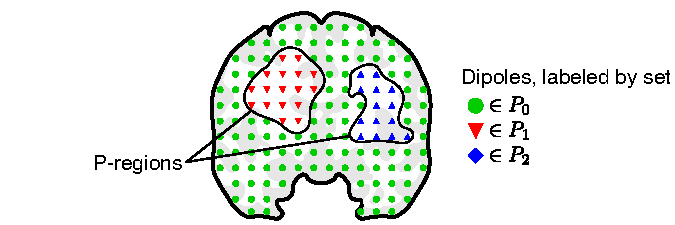
\includegraphics[width=0.65\linewidth]{./img/Pregions_pic}
\end{figure}
\end{frame}

\begin{frame}{Model Assumptions}
Sources are independent, but synchronized within each P-region
\begin{equation}
\text{Cov}\ppar{\SA\ppar{n_1}, \SA\ppar{n_2}}
=
\begin{cases}
\ppar{\theta_0+\theta_k}, &\text{if } n_1, n_2 \in P_k, k\neq 0 \\
\theta_0, &\text{if } n_1, n_2 \in P_0 \\
0, &\text{otherwise}.
\end{cases}
\end{equation}

Sources are thus separated into regionally synchronized activity, $\mathbf{R}$, and background activity, $\BA$,
\begin{equation}
    {\SA} + \varepsilon = {\BA} + \PA {\RA}
    = {\BA} + \sum_{k=1}^K \PA(:,k) {\RA}(k)
\end{equation}
\end{frame}

\begin{frame}{Model Assumptions}
Recall, the sources (to be estimated) are decomposed as
\begin{equation}
    {\SA} + \varepsilon = {\BA} + \PA {\RA}
    = {\BA} + \sum_{k=1}^K \PA(:,k) {\RA}(k)
\end{equation}

In the assumption of Gaussian noise, we have then
\begin{align}
    \BA &\sim \norm\ppar{0, \theta \id_N } 
     \\
    \RA &\sim \norm\ppar{0, 
    \spar{\text{diag}\ppar{\theta_1, \theta_2, \dots, \theta_K}} }
\end{align}
with $\theta_k \gg \theta_0$ for all $k$.
\end{frame}

\begin{frame}{Derivation of Estimator}
We use a Maximum A Posteriori Estimator,
\begin{align}
    \hat{\SA} &= 
    \argmax_{\SA }\, 
    \phantom{.}
    \log \ppar{
    \text{Prob}\ppar{ \Y \given \SA }\,  \text{Prob}\ppar{ \SA } }.
\end{align}

This lead to the following optimization problem,
\begin{align}
    \sset{ \hat{\BA}, \hat{\RA} } 
    =
    \argmax_{\BA, \RA }\, 
    &\phantom{.}
    \frac{\sigma}{2 \theta_0} \nnorm{\BA}^2
    +
    \sum_{k=1}^K \frac{1}{2\theta_k } \nnorm{\PA(:,k)\, \RA(k)}^2
    \nonumber \\
    \text{s.t.}
    \quad
    &\phantom{.}
    {\G \ppar{\BA + \PA \RA} } - \Y = 0
    \label{eq:3.7}
\end{align}
which is smooth.
\end{frame}

\begin{frame}{Derivation of Estimator}
The optimization problem \ref{eq:3.7} has the following Lagrangian function
\begin{align}
    \mathcal{L}\ppar{\BA, \RA, \lambda} &=
    \frac{1}{2 \theta_0} \nnorm{\BA}^2
    +
    \sum_{k=1}^K \frac{1}{2 \theta_k} \nnorm{\PA(:,k)\, \RA(k)}^2
    \nonumber \\
    &\phantom{=} \quad
    +
    \lambda^T \ppar{{\G \ppar{\BA + \PA \RA} } - \Y}
\end{align}

By solving the normal equations, $\ppar{\frac{\partial}{\partial \bullet}} \mathcal{L} = 0$, we obtain
\begin{align*}
    \hat{\SA}
    &=
    \ppar{ \theta_0 \id_N + \sum_{k=1}^K \theta_k \abss{P_k}^{-1} 
    \PA(:,k)\, \PA(:,k)^T
    } \G^T W_\rho \Y
    %\label{eq:3.24}
    \\
    W_\rho &=
    \spar{\G \ppar{ \theta_0 \id_N + \sum_{k=1}^K \theta_k \abss{P_k}^{-1} 
    \PA(:,k)\, \PA(:,k)^T
    } \G^T }^\dagger
    %\label{eq:3.25}
\end{align*}
\end{frame}

\begin{frame}{Derivation of Estimator}
For ease of notation, the parameter $\theta_0$ will be replaced by rewriting
\begin{align}
    \hat{\SA}
    &=
    \ppar{ \id_N + \sum_{k=1}^K \tau_k \abss{P_k}^{-1} 
    \PA(:,k)\, \PA(:,k)^T
    } \G^T W_\lambda \Y
    \label{eq:3.24}
    \\
    W_\lambda &=
    \spar{\G \ppar{ \id_N + \sum_{k=1}^K \tau_k \abss{P_k}^{-1} 
    \PA(:,k)\, \PA(:,k)^T
    } \G^T + \lambda \id_M }^{-1}
    \label{eq:3.25}
\end{align}
with $\tau_k = \theta_k/\theta_0$.
%
The regularization parameter $\lambda>0$ is introduced for stability of the inverse.
\end{frame}

\section{Results}

\begin{frame}{Protocol for Synthetic Data}
\begin{enumerate}
    \item Construct the leadfield matrix $\G$.
    \item Select a `seed' dipole, $n^*$.
    \item Construct source distribution, $\SA$, as
    \begin{equation}
\SA(n) = f\ppar{ \nnorm{\rr_n-\rr_{n^*}} / \kappa }.
\end{equation}
    \item Construct noiseless EEG measurements, $\Y_0 = \G \SA$.
    \item Construct some additive noise, $\varepsilon$, in order to achieve a prescribed Signal-to-Noise Ratio $\ppar{\text{SNR}_\text{dB}}$.
    \item Construct the EEG measurements, $\Y = \Y_0 + \varepsilon$.
\end{enumerate}
\end{frame}

\begin{frame}{Shape of Source Patch}
This factor was surprisingly important.
\begin{align}
\text{Square} &&
    f_\text{sq}(x) 
    &= 
    \begin{cases}
1, &\text{if } x\leq 1 \\
0, &\text{otherwise}.
\end{cases}
    \\
\text{Gaussian} &&
    f_\text{Gauss}(x) 
    &= 
    e^{-x^2/\kappa}
    \\
\text{Exponential} &&
    f_\text{exp}(x) 
    &= 
    e^{-x/\kappa}
    \\
\text{Polynomial} &&
    f_\text{pol}(x) 
    &= 
    \sqrt{ \max \sset{1-{x}^2, 0 }}
\end{align}
\end{frame}

\begin{frame}{Shape of Source Patch}
This factor was surprisingly important.
\begin{figure}
\centering
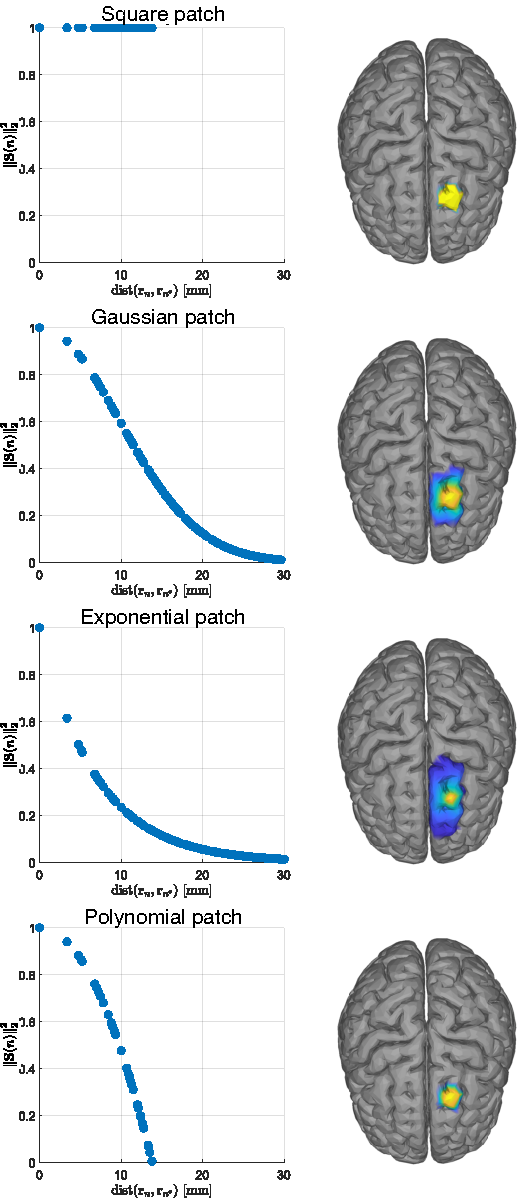
\includegraphics[width=0.8\linewidth]{./img/profiles.pdf}
\end{figure}
\end{frame}

{
%\metroset{background=dark}
\subsection{Synthetic Data (Human)}
}

\begin{frame}{Synthetic Data: Human Model}
\begin{itemize}
\item Subject: ICBM152 human MRI template. This is the `average' of 152 subjects \cite{icbm152_2011}.
\item $M=90$ EEG electrodes according to the 10-10 International System.
\item $N=15,002$ constrained equivalent dipoles on the brain cortex.
\item 4-sphere model with (1) brain, (2) CSF, (3) skull, and (4) head. 
\end{itemize}
\end{frame}

\begin{frame}{Synthetic Data: Human Model}
\begin{figure}
\centering
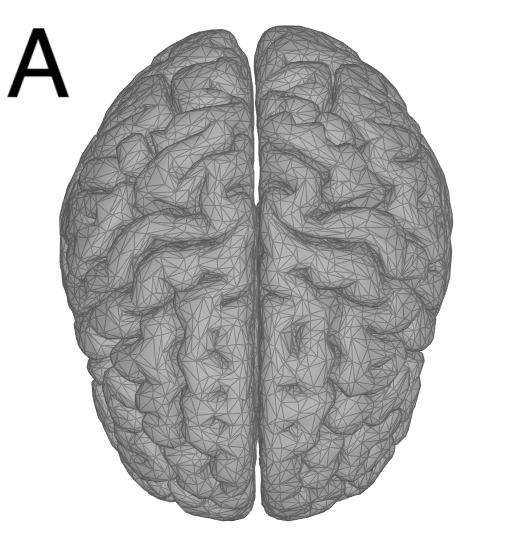
\includegraphics[width=0.18\linewidth]{./img_dev/3D_Subject_ICBM152_2019b_top - Copy2}
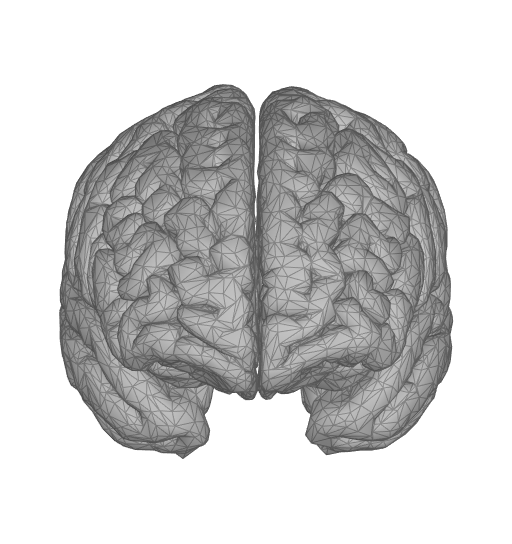
\includegraphics[width=0.18\linewidth]{./img_dev/3D_Subject_ICBM152_2019b_front}
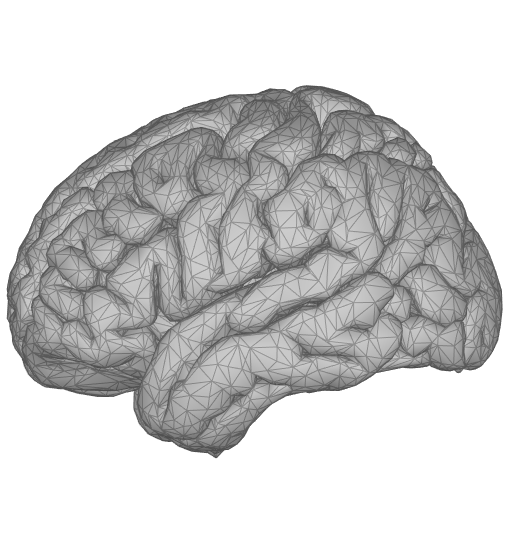
\includegraphics[width=0.18\linewidth]{./img_dev/3D_Subject_ICBM152_2019b_left}
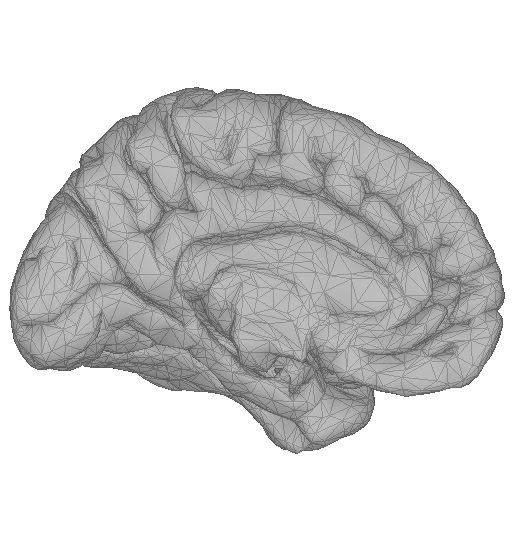
\includegraphics[width=0.18\linewidth]{./img_dev/3D_Subject_ICBM152_2019b_left_inner}
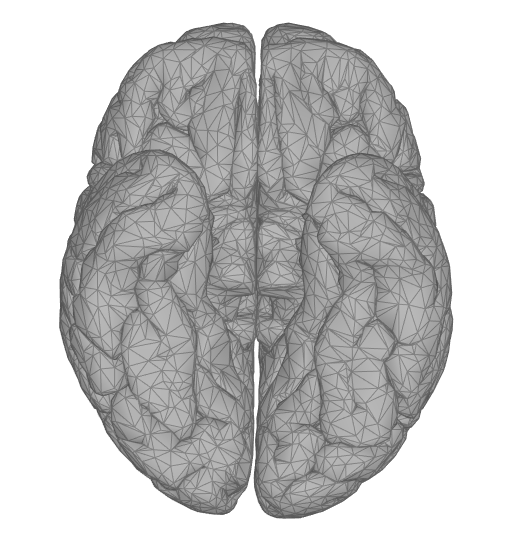
\includegraphics[width=0.18\linewidth]{./img_dev/3D_Subject_ICBM152_2019b_bottom}
%
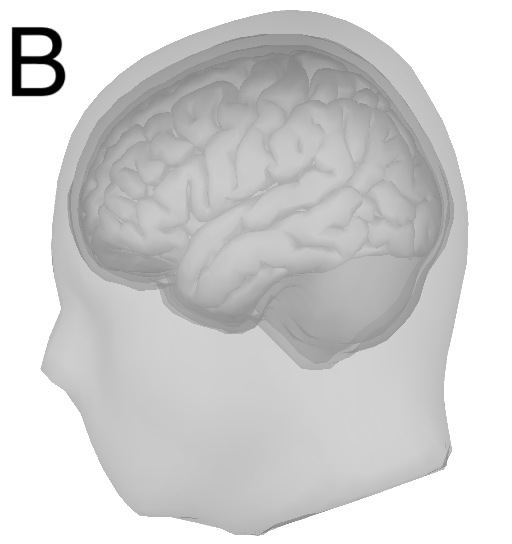
\includegraphics[width=0.18\linewidth]{./img_dev/combined - Copy}
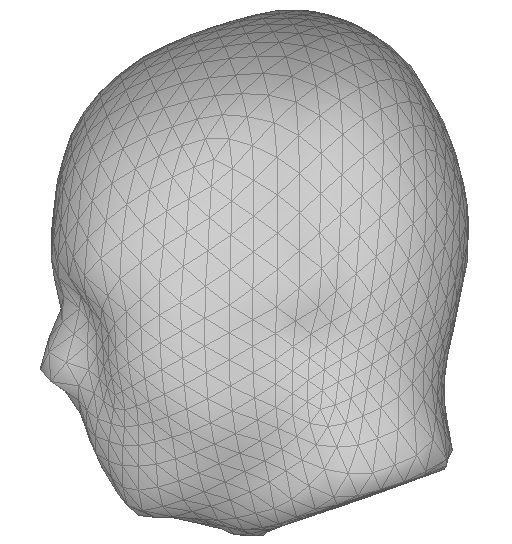
\includegraphics[width=0.18\linewidth]{./img_dev/combined_scalp}
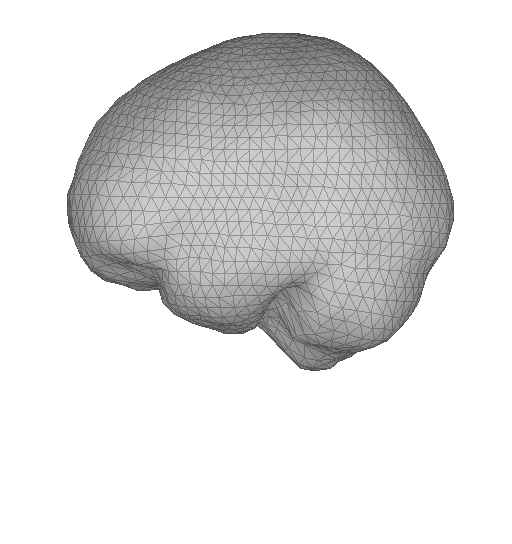
\includegraphics[width=0.18\linewidth]{./img_dev/combined_skull_outer}
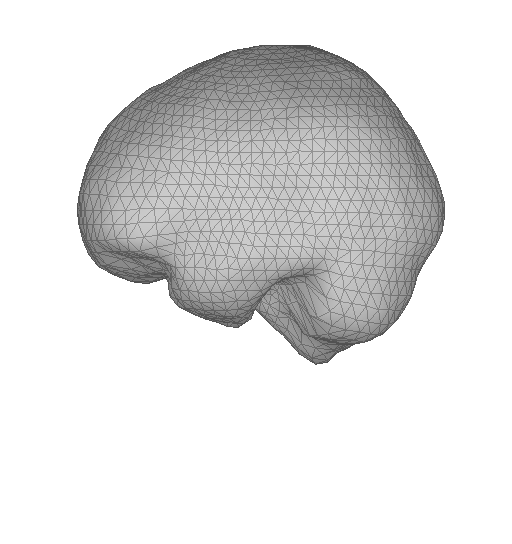
\includegraphics[width=0.18\linewidth]{./img_dev/combined_skull_inner}
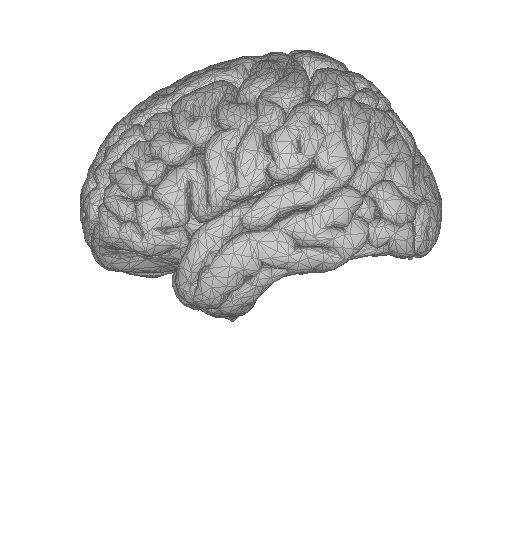
\includegraphics[width=0.18\linewidth]{./img_dev/combined_cortex}
\end{figure}
\end{frame}

\begin{frame}{Synthetic Data: Human Model}
\begin{figure}
\centering
\includegraphics[width=0.8\linewidth]{./img/EEG_10-10.pdf}
\end{figure}
\end{frame}

\begin{frame}{Synthetic Data (Human)}
In order to use the proposed method, one single P-region is constructed for each trial following these steps:
\begin{enumerate}
    \item Recall the position of the seed dipole, $\rr_{n^*}$. The source patch has an approximate radius of $\kappa = 12.6$ mm.
    \item Select a point at the cortex, $\mathbf{c}$, so that $\nnorm{\rr_{n^*}-\mathbf{c}}< \kappa$.
    \item Region $P_1$ consist on a ball with center at $\mathbf{c}$ an radius $2\kappa$.
    \item Region $P_0$ comprises all dipoles not in $P_1$.
\end{enumerate}
\end{frame}

\begin{frame}{Synthetic Data (Human)}
General performance
\begin{figure}
    \centering
    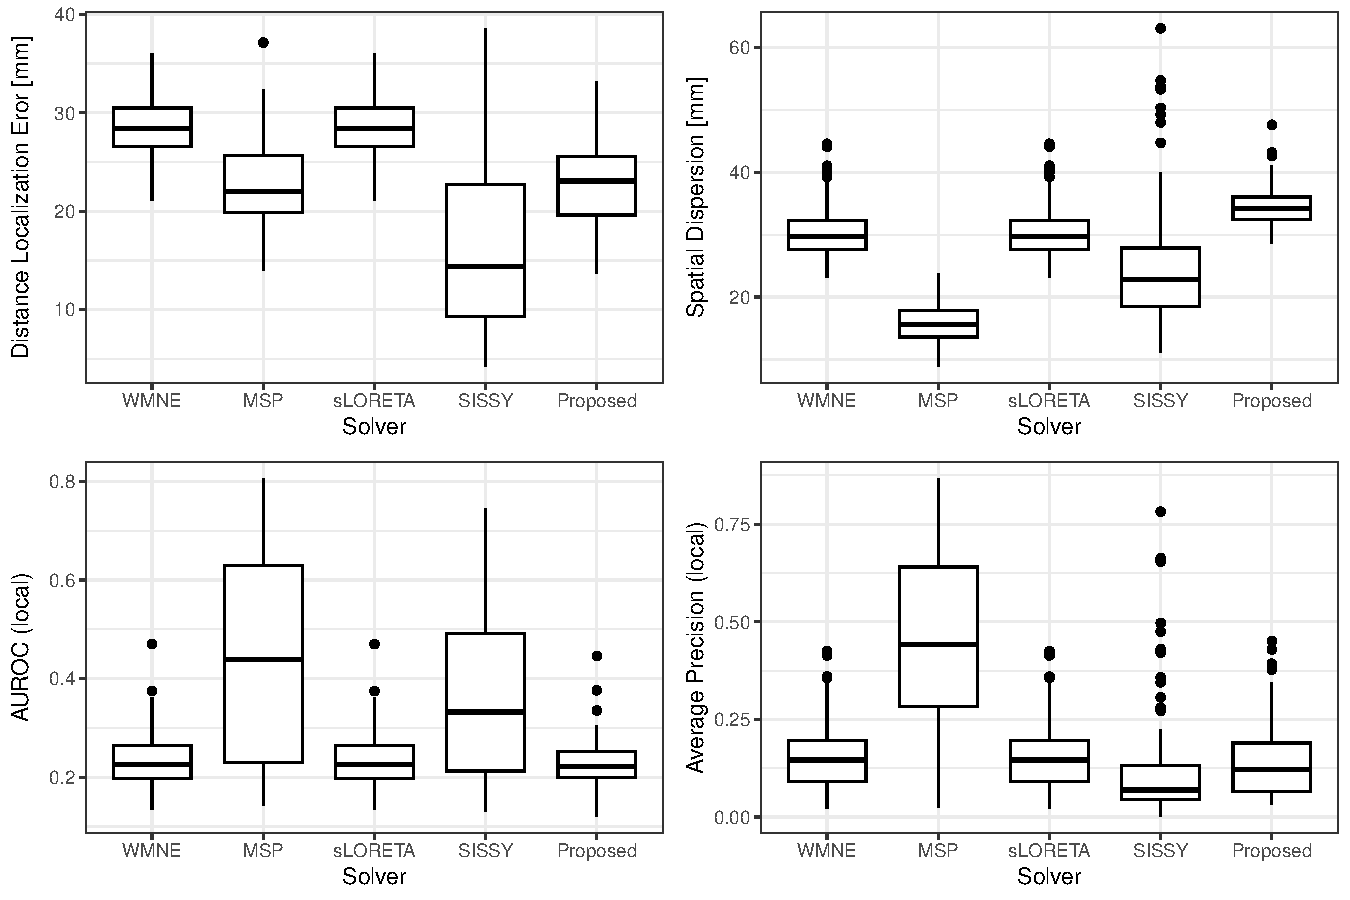
\includegraphics[width=0.7\linewidth]{img_stats/P_plot_EvalMetrics_Protocol04_30ALL.pdf}
\end{figure}
\end{frame}

\begin{frame}{Synthetic Data (Human)}
Pearson correlation of variables
\begin{table}[]
\centering
\begin{tabular}{@{}lllll@{}}
\toprule
      & SD    & AUROC & AP    & Depth  \\
\midrule
DLE   & 0.733 & -0.477 & -0.054 & -0.097 \\
SD    &       & -0.555 & -0.393 & 0.079  \\
AUROC &       &        & 0.536  & -0.103 \\
AP    &       &        &        & -0.108 \\
\bottomrule
\end{tabular}
\end{table}
\end{frame}

\begin{frame}{Synthetic Data (Human)}
General performance, accounting for shape of source patch
\begin{figure}
    \centering
    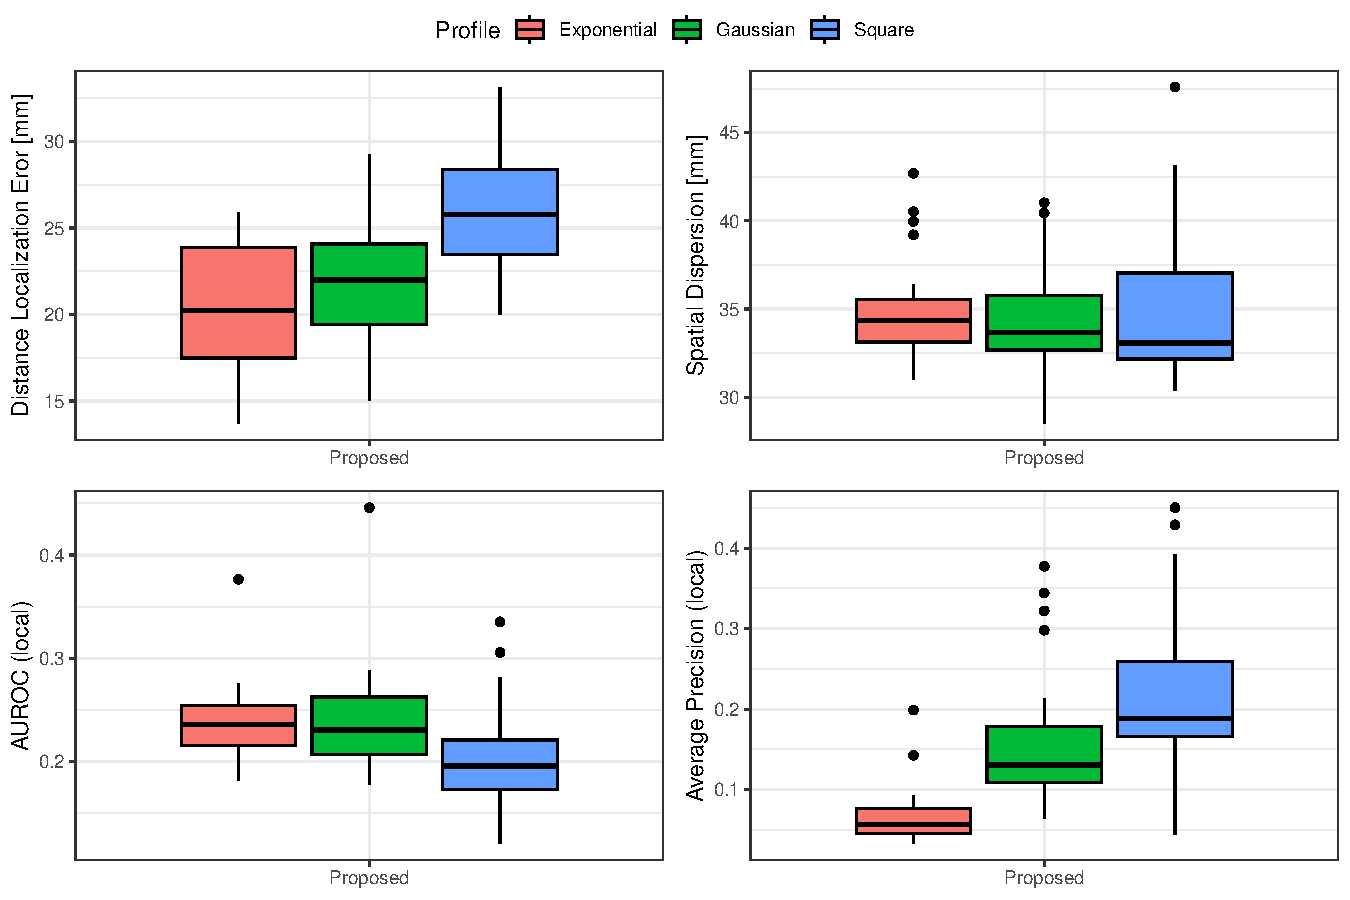
\includegraphics[width=0.7\linewidth]{img_stats/P_shape_EvalMetrics_Protocol04_30ALL.pdf}
\end{figure}
\end{frame}

\begin{frame}{Synthetic Data (Human)}
General performance degradation due to noise
\begin{figure}
    \centering
    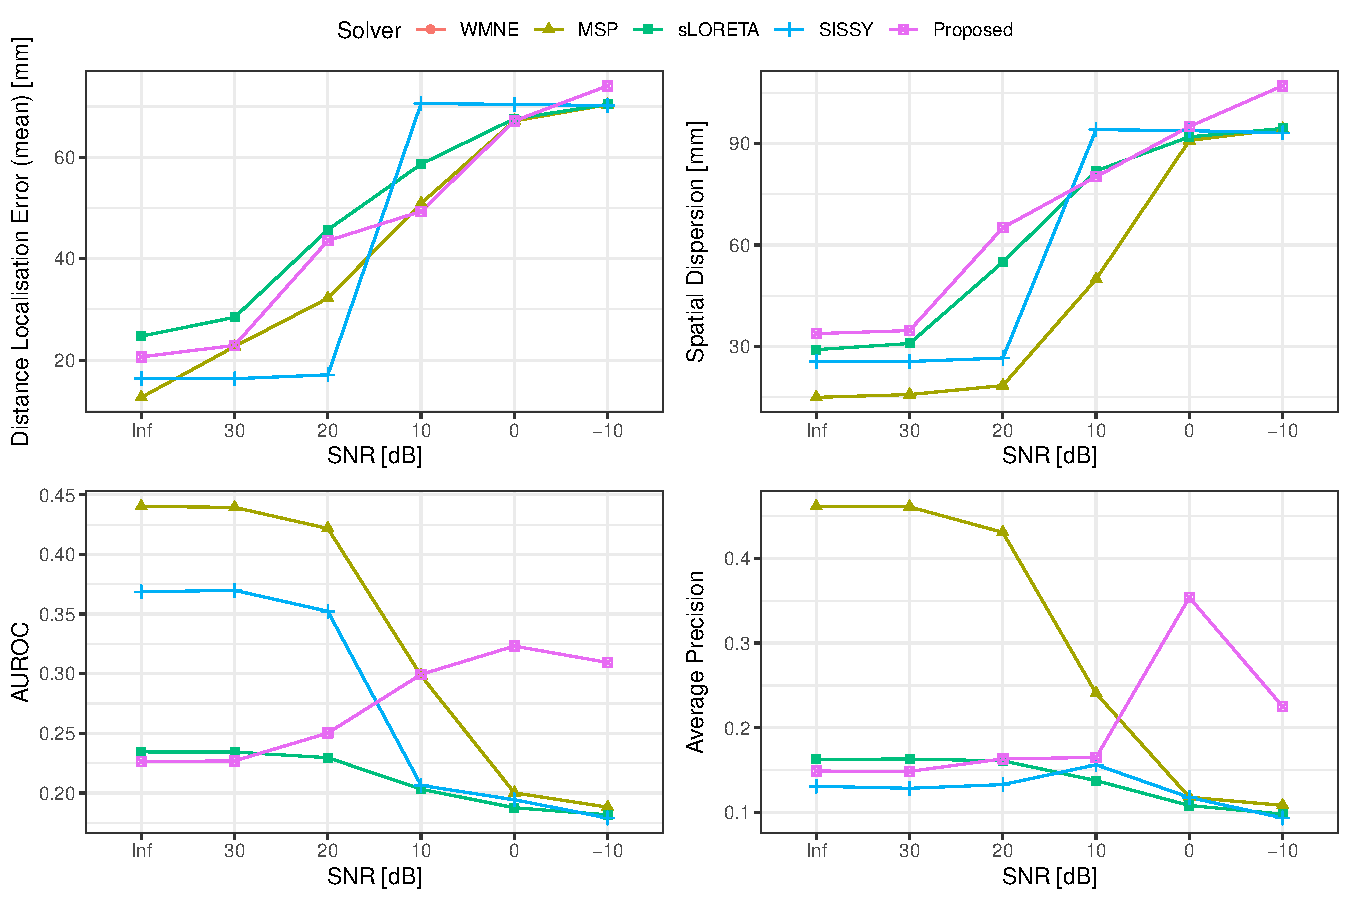
\includegraphics[width=0.7\linewidth]{img_stats/P_SNRdegradation_EvalMetrics_Protocol04_30.pdf}
\end{figure}
\end{frame}


{
%\metroset{background=dark}
\subsection{Synthetic Data (Animal)}
}


\begin{frame}{Synthetic Data: Animal Model}
\begin{itemize}
\item Subject: young male Yucatan minipig (\textit{Sus scrofa}).
\item Age-matched publicly available MRI template by Joanne et al. \cite{pig_template}.
\item $M=8$ surface electrodes at cortex surface.
\item $N=4,940$ unconstrained equivalent dipoles on an adaptive grid over the brain volume.
\item 2-sphere model with (1) brain and (2) cortex envelope. 
\end{itemize}
\end{frame}

\begin{frame}{Synthetic Data: Animal Model}
\begin{figure}
\centering
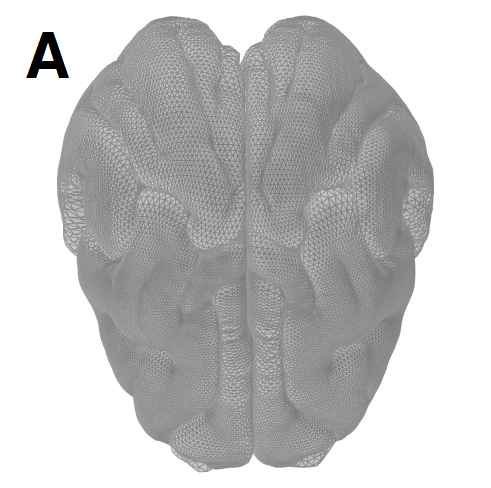
\includegraphics[width=0.18\linewidth]{./img_dev2/3D_subject17_top}
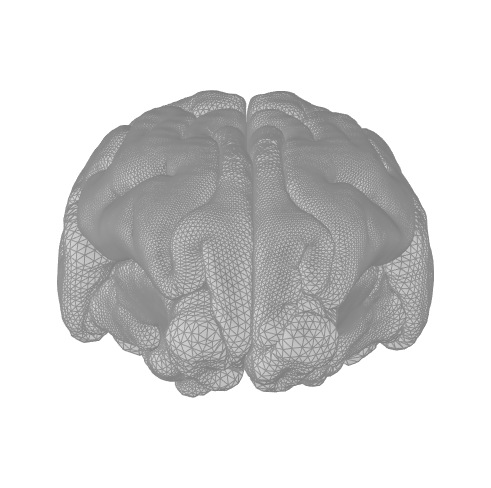
\includegraphics[width=0.18\linewidth]{./img_dev2/3D_subject17_front}
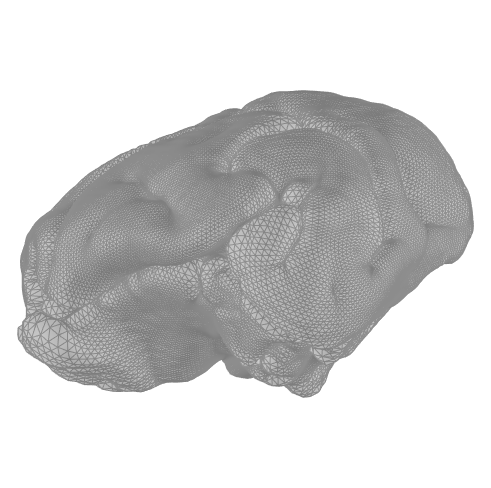
\includegraphics[width=0.18\linewidth]{./img_dev2/3D_subject17_left}
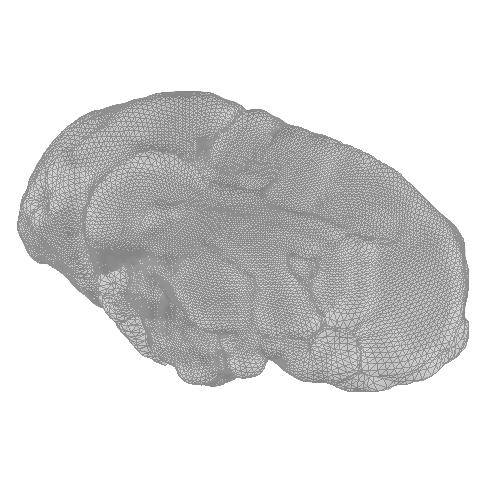
\includegraphics[width=0.18\linewidth]{./img_dev2/3D_subject17_left_in}
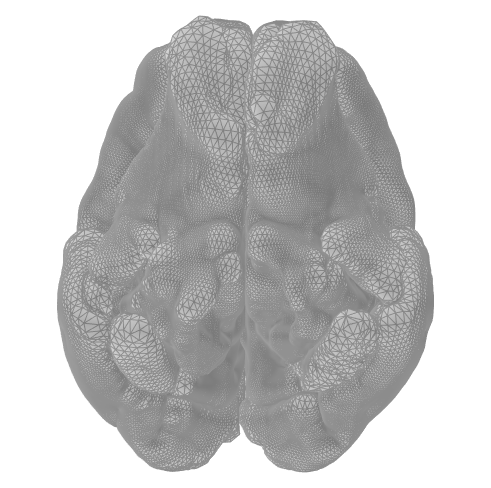
\includegraphics[width=0.18\linewidth]{./img_dev2/3D_subject17_bottom}
%
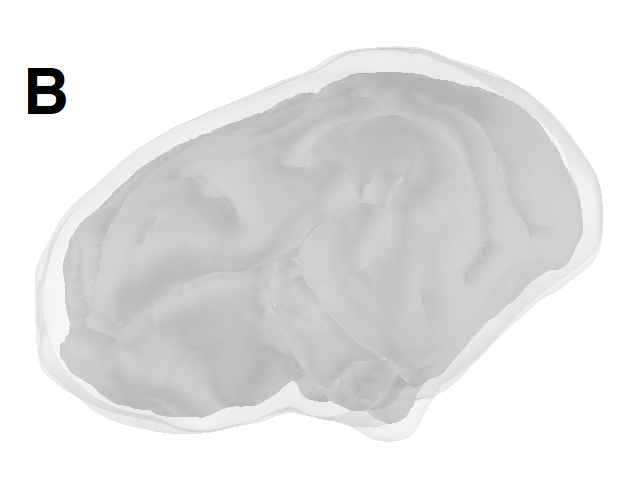
\includegraphics[width=0.23\linewidth]{./img_dev2/3D_subject17_compositeA}
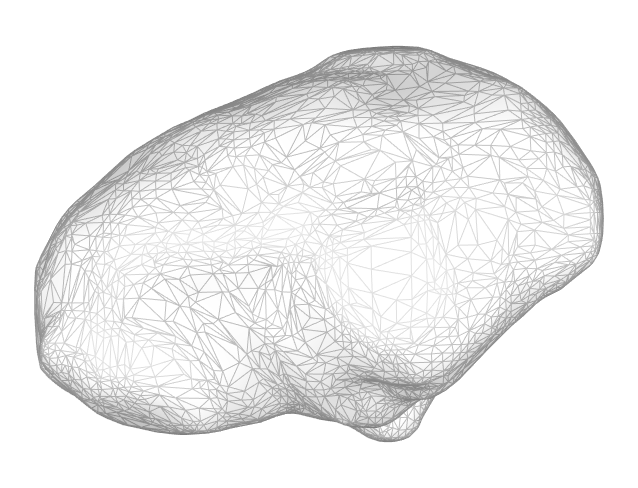
\includegraphics[width=0.23\linewidth]{./img_dev2/3D_subject17_compositeB}
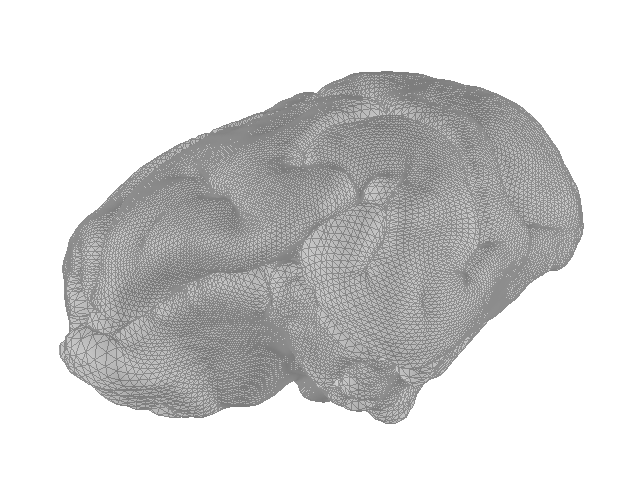
\includegraphics[width=0.23\linewidth]{./img_dev2/3D_subject17_compositeC}
\end{figure}
\end{frame}

\begin{frame}{Synthetic Data: Animal Model}
\begin{figure}
\centering
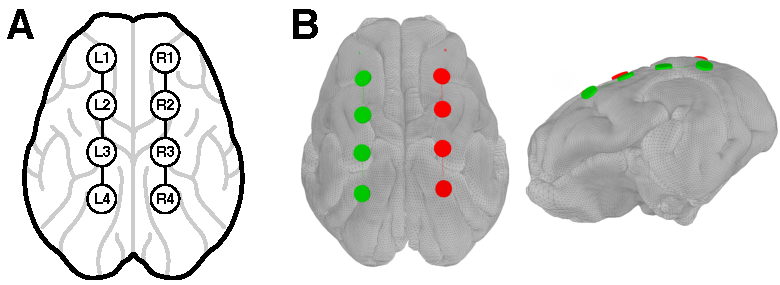
\includegraphics[width=0.8\linewidth]{./img/electrodes_pig.pdf}
\end{figure}
\end{frame}

\begin{frame}{Synthetic Data (Animal)}
A single P-region is constructed per each trial, following the same protocol with $\kappa =$ 8.95 mm.\\

This value of $\kappa$ was selected so that the resulting source patches have an approximate volume of 3 $\text{cm}^3$, which is similar to the volume of the region with pathological symptoms observed in the real data.
\end{frame}

\begin{frame}{Synthetic Data (Animal)}
General performance
\begin{figure}
    \centering
    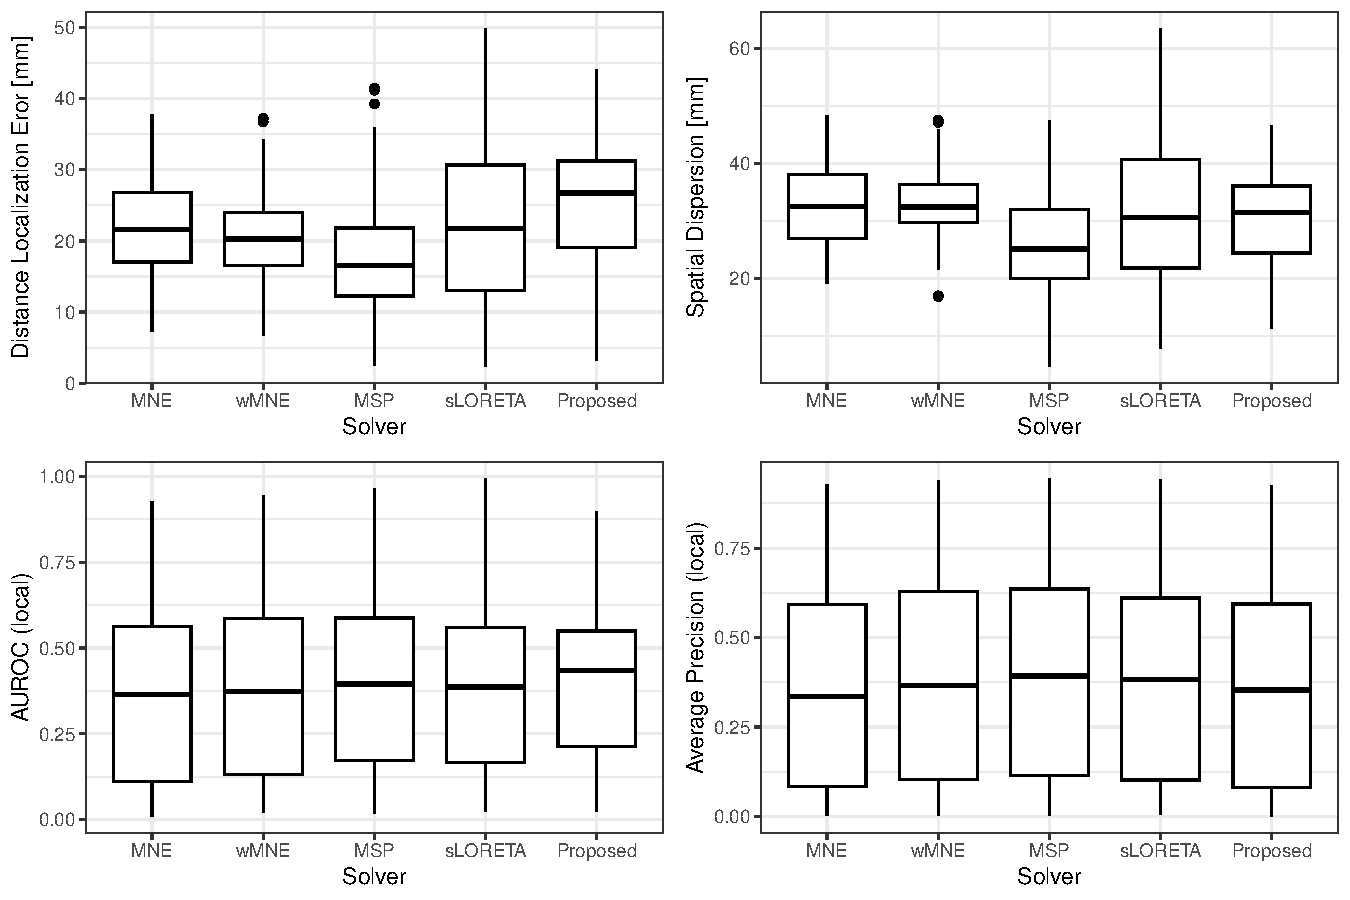
\includegraphics[width=0.7\linewidth]{img_stats/pig_plot_EvalMetrics_protocol04_vol5k_pigALL.pdf}
\end{figure}
\end{frame}

\begin{frame}{Synthetic Data (Animal)}
Pearson correlation of variables
\begin{table}[]
\centering
\begin{tabular}{@{}lllll@{}}
\toprule
      & SD    & AUROC & AP    & Depth  \\
\midrule
DLE   & 0.870 & 0.138 & 0.105 & -0.192 \\
SD    &       & 0.028 & 0.008 & -0.144 \\
AUROC &       &       & 0.957 & -0.035 \\
AP    &       &       &       & -0.063 \\
\bottomrule
\end{tabular}
\end{table}
\end{frame}

\begin{frame}{Synthetic Data (Animal)}
General performance, accounting for shape of source patch
\begin{figure}
    \centering
    \includegraphics[width=0.7\linewidth]{img_stats/pig_shape_EvalMetrics_Protocol04_vol5k_pigALL.pdf}
\end{figure}
\end{frame}

\begin{frame}{Synthetic Data (Animal)}
General performance degradation due to noise
\begin{figure}
    \centering
    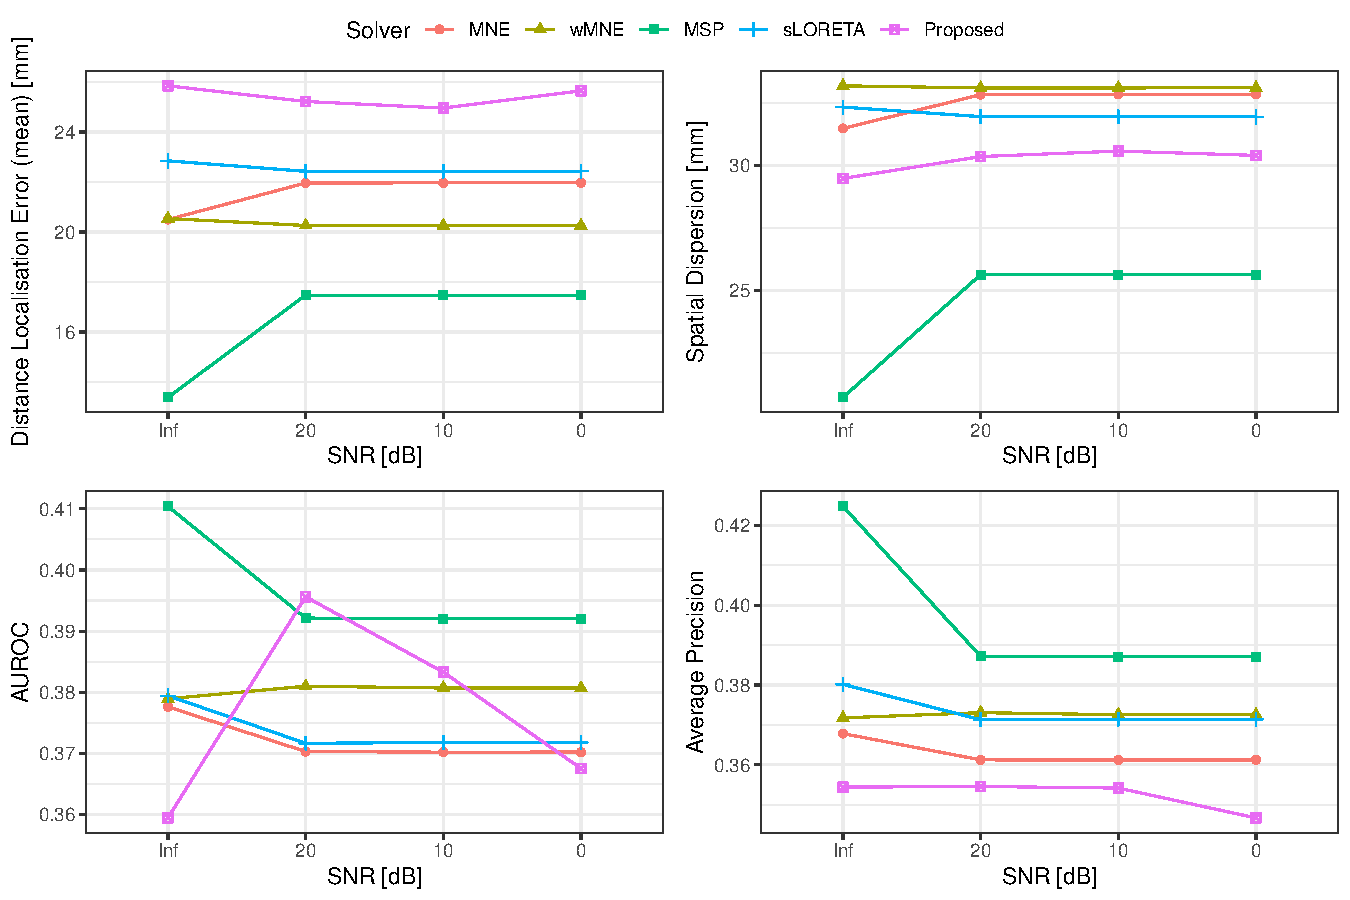
\includegraphics[width=0.7\linewidth]{img_stats/pig_SNRdegradation_EvalMetrics_protocol04_vol5k_pig.pdf}
\end{figure}
\end{frame}

{
%\metroset{background=dark}
\subsection{Real Data}
}

\begin{frame}{Real Data}
The proposed ESI method is used on a real dataset from an experiment by Pascual et al. \footfullcite{pig_lesion1, PMID_36109613} at UT Southwestern.\\

Acute Ischemic Stroke was induced in the subject by obstruction of the Middle
Cerebral Artery. Stroke is the obstruction of a vein or artery in the
brain, which stops the supply of oxygenated blood.\\

 The brain regions affected by
hypoxia (lack of oxygen at a cellular level) are called the Ischemic Penumbra.
\end{frame}

\begin{frame}{Pathology Data}
During a post-mortem analysis, the subject's brain was extracted and sliced in order to be stained with 
triphenyltetrazolium (TTC).\\

TTC staining is used to identify the Ischemic Penumbra, which is used to define the P-region $P_1$.

\begin{figure}
\centering
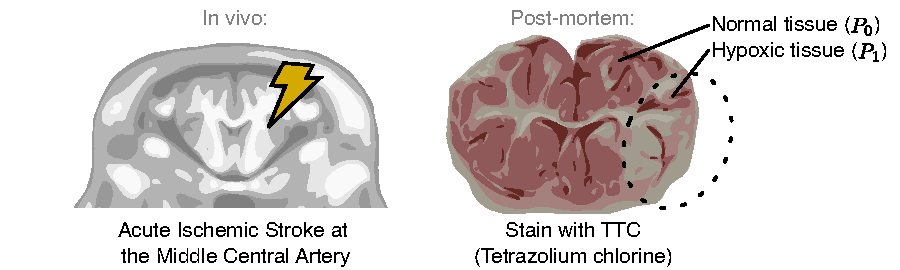
\includegraphics[width=0.8\linewidth]{./img/Pregions_real}
\end{figure}
\end{frame}

\begin{frame}{Results (Real Data)}
Time series with ECoG recordings; induced lesion happened at $t=0$ s.
\begin{figure}
\centering
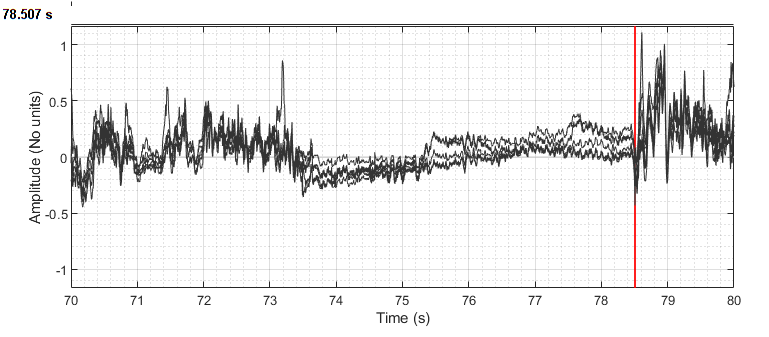
\includegraphics[width=0.9\linewidth]{./img_dev2/ECOG_All_sub17diss_diss1}
\end{figure}
\end{frame}

\begin{frame}{Results (Real Data)}
Normalized source activations, $\nnorm{\hat{S}(n)}_2/\max\sset{\nnorm{\hat{S}(n)}_2}$, superimposed with MRI.
\begin{figure}
\centering
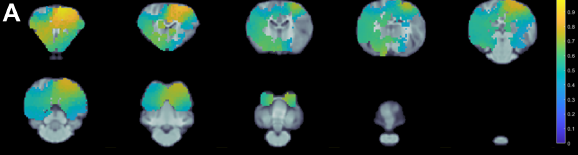
\includegraphics[width=0.99\linewidth]{./img_dev3/proposed_A}
\end{figure}
\textbf{wMNE}
\end{frame}

\begin{frame}{Results (Real Data)}
Normalized source activations, $\nnorm{\hat{S}(n)}_2/\max\sset{\nnorm{\hat{S}(n)}_2}$, superimposed with MRI.
\begin{figure}
\centering
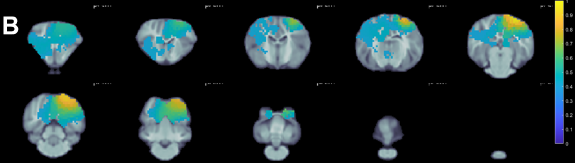
\includegraphics[width=0.99\linewidth]{./img_dev3/proposed_B}
\end{figure}
\textbf{MSP}
\end{frame}

\begin{frame}{Results (Real Data)}
Normalized source activations, $\nnorm{\hat{S}(n)}_2/\max\sset{\nnorm{\hat{S}(n)}_2}$, superimposed with MRI.
\begin{figure}
\centering
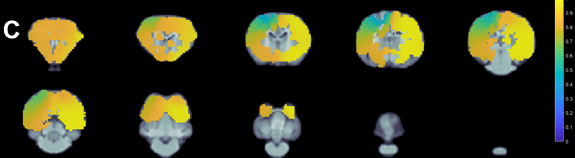
\includegraphics[width=0.99\linewidth]{./img_dev3/proposed_C}
\end{figure}
\textbf{sLORETA}
\end{frame}

\begin{frame}{Results (Real Data)}
Normalized source activations, $\nnorm{\hat{S}(n)}_2/\max\sset{\nnorm{\hat{S}(n)}_2}$, superimposed with MRI.
\begin{figure}
\centering
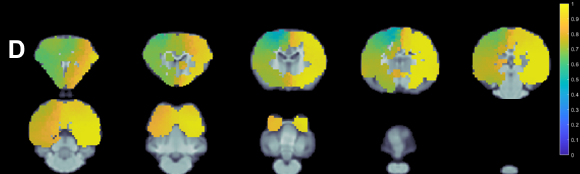
\includegraphics[width=0.99\linewidth]{./img_dev3/proposed_D}
\end{figure}
\textbf{Proposed method}
\end{frame}

\begin{frame}{Acknowledgements}
\begin{itemize}
\item To Dr. Jianzhong Su for his encouragement and support.
\item To the members of my dissertation committee: Dr. Hristo V. Kojouharov, Dr. Ren-Cang Li, and Dr. Li Wang.
\item To Imelda Trejo-Lorenzo for her encouragement, help, and guidance.
\item To the colleagues I met at UTA, and the friends from home who are family in my heart.
\item To my family: my brother E. Ricardo, my mother Mar\'ia Guadalupe, and my late father Nicol\'as.
\end{itemize}
\end{frame}

\begin{frame}{Thanks for your attention}

\end{frame}

%{
%%\metroset{background=dark}
%\section{Bibliography}
%}

%\begin{frame}[allowframebreaks]
%        \frametitle{References}
%\bibliographystyle{abbrv} % We choose the "plain" reference style
%%\bibliography{./refs_old} % Entries are in the refs.bib file
%\bibliography{./refs} % Entries are in the refs.bib file
%\end{frame}

\begin{frame}[allowframebreaks]
  \frametitle{References}
  \printbibliography
\end{frame}

\end{document}